\documentclass{article}

\usepackage{filecontents}
\usepackage{tikz}
\usepackage{amsmath}
\usepackage{amsfonts}
\usepackage[bookmarks=true]{hyperref}

\def\R{\ensuremath{\mathbb{R}}}
\begin{filecontents}{tmp.bib}
@book{boyd,
  title={\href{http://stanford.edu/~boyd/cvxbook/}{Convex Optimization}},
  author={Boyd, Stephen and Vandenberghe, Lieven},
  year={2004},
  publisher={Cambridge university press}
}

\end{filecontents}

\begin{document} 

\section{The maximum ball on a surface element of a polytope as a convex
optimization problem} 
%%%%%%%%%%%%%%%%%
\begin{figure}[h]
\centering
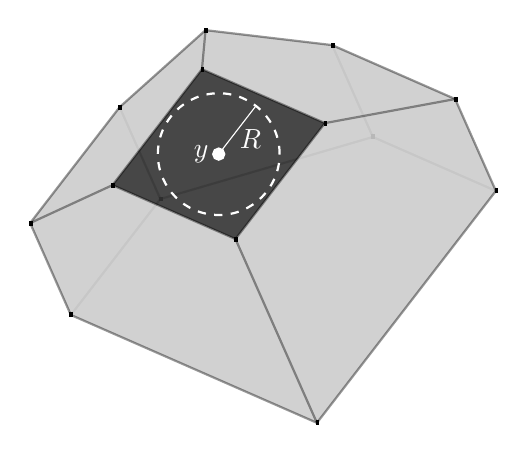
\begin{tikzpicture}%
        [x={(0.258520cm, -0.583496cm)},
        y={(0.781193cm, -0.342529cm)},
        z={(-0.568247cm, -0.736347cm)},
        scale=2.000000,
        back/.style={loosely dotted, thin},
        edge/.style={color=black, thick, opacity=0.4},
        circle/.style={color=white, thick, dashed},
        facet/.style={fill=black!20,color=black!20,fill opacity=0.9},
        specialFacet/.style={fill=black!20,color=black!80,fill opacity=0.9},
        vertex/.style={inner sep=0.5pt,circle,draw=black!25!black,fill=black!75!black,thick,anchor=base},
        vertexC/.style={inner sep=5pt,circle,draw=black!100!black,fill=black!100!black,thick,anchor=base}]
%
%
%% Coordinate of the vertices:
%%

\coordinate (0.5, 0.5, -1.05) at (0.5, 0.5, 1.05);

\coordinate (-0.500, -0.500, -0.500) at (-0.500, -0.500, -0.500);
\coordinate (-1.00, 0.000, 0.000) at (-1.00, 0.000, 0.000);
\coordinate (-1.00, 0.000, 1.00) at (-1.00, 0.000, 1.00);
\coordinate (-1.00, 1.00, 0.000) at (-1.00, 1.00, 0.000);
\coordinate (-1.00, 1.00, 1.00) at (-1.00, 1.00, 1.00);
\coordinate (0.000, -1.00, 0.000) at (0.000, -1.00, 0.000);
\coordinate (0.000, -1.00, 1.00) at (0.000, -1.00, 1.00);
\coordinate (0.000, 0.000, -1.00) at (0.000, 0.000, -1.00);
\coordinate (0.000, 1.00, -1.00) at (0.000, 1.00, -1.00);
\coordinate (1.00, -1.00, 0.000) at (1.00, -1.00, 0.000);
\coordinate (1.00, -1.00, 1.00) at (1.00, -1.00, 1.00);
\coordinate (1.00, 0.000, -1.00) at (1.00, 0.000, -1.00);
\coordinate (1.00, 1.00, -1.00) at (1.00, 1.00, -1.00);
\coordinate (1.00, 1.00, 1.00) at (1.00, 1.00, 1.00);
%%
%%
%% Drawing edges in the back
%%
%%
%%
%% Drawing vertices in the back
%%
\node[vertex] at (1.00, -1.00, 0.000)     {};
\node[vertex] at (1.00, 0.000, -1.00)     {};
%%
%%
%% Drawing the facets
%%
\draw[edge] (0.000, -1.00, 0.000) -- (1.00, -1.00, 0.000);
\draw[edge] (0.000, 0.000, -1.00) -- (1.00, 0.000, -1.00);
\draw[edge] (1.00, 0.000, -1.00) -- (1.00, 1.00, -1.00);
\draw[edge] (1.00, -1.00, 0.000) -- (1.00, -1.00, 1.00);
\draw[edge] (1.00, -1.00, 0.000) -- (1.00, 0.000, -1.00);

\fill[facet] (1.00, 1.00, 1.00) -- (-1.00, 1.00, 1.00) -- (-1.00, 1.00, 0.000) -- (0.000, 1.00, -1.00) -- (1.00, 1.00, -1.00) -- cycle {};
\fill[facet] (1.00, 1.00, 1.00) -- (-1.00, 1.00, 1.00) -- (-1.00, 0.000, 1.00) -- (0.000, -1.00, 1.00) -- (1.00, -1.00, 1.00) -- cycle {};
\fill[facet] (0.000, -1.00, 1.00) -- (-1.00, 0.000, 1.00) -- (-1.00, 0.000, 0.000) -- (-0.500, -0.500, -0.500) -- (0.000, -1.00, 0.000) -- cycle {};
\fill[facet] (0.000, 1.00, -1.00) -- (-1.00, 1.00, 0.000) -- (-1.00, 0.000, 0.000) -- (-0.500, -0.500, -0.500) -- (0.000, 0.000, -1.00) -- cycle {};
\fill[specialFacet] (-1.00, 1.00, 1.00) -- (-1.00, 0.000, 1.00) -- (-1.00, 0.000, 0.000) -- (-1.00, 1.00, 0.000) -- cycle {};
\draw[edge] (1.00, -1.00, 1.00) -- (1.00, 1.00, 1.00);
\draw[edge] (1.00, 1.00, -1.00) -- (1.00, 1.00, 1.00);
\draw[edge] (0.000, -1.00, 1.00) -- (1.00, -1.00, 1.00);
\draw[edge] (0.000, 0.000, -1.00) -- (0.000, 1.00, -1.00);
\draw[edge] (0.000, 1.00, -1.00) -- (1.00, 1.00, -1.00);
%%
%%
%% Drawing edges in the front
%%
\draw[edge] (-0.500, -0.500, -0.500) -- (-1.00, 0.000, 0.000);
\draw[edge] (-0.500, -0.500, -0.500) -- (0.000, -1.00, 0.000);
\draw[edge] (-0.500, -0.500, -0.500) -- (0.000, 0.000, -1.00);
\draw[edge] (-1.00, 0.000, 0.000) -- (-1.00, 0.000, 1.00);
\draw[edge] (-1.00, 0.000, 0.000) -- (-1.00, 1.00, 0.000);
\draw[edge] (-1.00, 0.000, 1.00) -- (-1.00, 1.00, 1.00);
\draw[edge] (-1.00, 0.000, 1.00) -- (0.000, -1.00, 1.00);
\draw[edge] (-1.00, 1.00, 0.000) -- (-1.00, 1.00, 1.00);
\draw[edge] (-1.00, 1.00, 0.000) -- (0.000, 1.00, -1.00);
\draw[edge] (-1.00, 1.00, 1.00) -- (1.00, 1.00, 1.00);
\draw[edge] (0.000, -1.00, 0.000) -- (0.000, -1.00, 1.00);
%%
%%
%% Drawing the vertices in the front
%%
\node[vertex] at (-0.500, -0.500, -0.500)     {};
\node[vertex] at (-1.00, 0.000, 0.000)     {};
\node[vertex] at (-1.00, 0.000, 1.00)     {};
\node[vertex] at (-1.00, 1.00, 0.000)     {};
\node[vertex] at (-1.00, 1.00, 1.00)     {};
\node[vertex] at (0.000, -1.00, 0.000)     {};
\node[vertex] at (0.000, -1.00, 1.00)     {};
\node[vertex] at (0.000, 0.000, -1.00)     {};
\node[vertex] at (0.000, 1.00, -1.00)     {};
\node[vertex] at (1.00, -1.00, 1.00)     {};
\node[vertex] at (1.00, 1.00, -1.00)     {};
\node[vertex] at (1.00, 1.00, 1.00)     {};
%%
\draw[circle] (-1.00, 0.50, 0.50) circle (11pt);
\draw[thick,fill=white,color=white!80] (-1.00, 0.500, 0.500) circle (1pt) node[left] {$y$};

\draw[fill=white,color=white] (-1.00, 0.500, 0.50) -- (-1.0,0.5,0.08) node[pos=0.3,right]{$R$};

\end{tikzpicture}
\caption{A polytope in $\R^3$ (light gray) and a surface element (dark gray). The goal is to find the largest inscribed circle (white) on top of the surface element.}
\end{figure}


Let us start with considering the problem of finding the
maximum ball $\mathcal{B}_R=\{x \in \R^N | \|x\| \leq R\}$, inside a polytope
$\mathcal{P} = \{x \in \R^N| a_i^T x \leq b_i, i=1,\cdots,M\}$.  As explained in
\cite{boyd}, this problem can be formulated as a linear programming problem.
The main insight is: Each hyperplane of the polytope can be seen as a
tangentialplane for a specific ball radius. The shortest distance between the
tangentialplane and the center of the ball is given by the radius multiplied by
the normal of the plane. Ergo to see if the ball is inside of the halfspace
defined by the hyperplane, we need to check the shortest distance only. Let us
denote this intersection of ball with hyperplane normal as $v_i = y +
R\frac{a_i}{\|a_i\|}$, with $y$ being the center of the ball. Now, intuitively the ball is
inside of the polytope iff each $v_i$ is inside of the polytope, meaning we need
to have the inequalities $a_i^Tv_i \leq b_i$ fulfilled. This gives us the linear programming formulation which can be found in \cite{boyd}:

\begin{equation}
        \begin{aligned}
                &\underset{y \in \R^N, R \in \R}{\text{maximize }}&&R\\
                &\text{subject to }&& a_i^T y + R\|a_i\|_2 \leq b_i\\
                &&& R \geq 0
        \end{aligned}
\end{equation}

Let us now consider the problem of finding the maximum ball in dimension $N-1$, $\mathcal{B}_R=\{x
\in \R^{N-1} | \|x\| \leq R\}$, restricted to a surface element of $\mathcal{P}$, which we denote as
\begin{center}
$\mathcal{S} = \{x \in \R^N| a_p^Tx=b_p, a_i^T x \leq b_i, i=1,\cdots,p-1,p+1,\cdots,M\}$
\end{center}

Meaning, the surface element $a_p^Tx=b_p$ will be intersected by the other
hyperplanes, which essentially makes this problem a lowerdimensional one. Since
we are operating on our surface element, we are interested in finding the normal
vectors, lying on the surface and pointing towards the intersection of the other
hyperplanes. Meaning, instead of having $v_i = y + R\frac{a_i}{\|a_i\|}$, we
need to find the orthogonal projection of $a_i$ onto the surface element, which
we get by $v_i = y + R\frac{a_i'}{\|a_i'\|}$ with $a_i' = a_i -
(a_i^Ta_p)a_p$ being the orthogonal projected vector. The resulting
linear optimization problem is

\begin{equation}
        \begin{aligned}
                &\underset{y \in \R^n, r \in \R}{\text{maximize }}&&R\\
                &\text{subject to }&& a_i^T y + R
                 \frac{a_i^T a_i'}{\|a_i'\|}\leq b_i,\\
                 &&&i\in \{1,\cdots,p-1,p+1,\cdots,m\}\\
                &&& a_i' = a_i - (a_i^Ta_p)a_p\\
                &&& a_p^Ty = b_p\\
                &&& R \geq 0
        \end{aligned}
\end{equation}
        whereby $R$ is the radius of the circle, $y$ the center, $a_i'$ is the
                orthogonal projection onto the hyperplane of $a_p$.




\bibliographystyle{plainnat}
\bibliography{tmp} 
\end{document}

